% !TEX TS-program = Xelatex
% !TEX encoding = UTF-8 Unicode

\documentclass[UTF8]{ctexart}
\usepackage{amsmath}
\usepackage[bottom]{footmisc}
\usepackage{geometry}
\usepackage{hyperref}
\usepackage{graphicx}
\usepackage{figsize}
\usepackage[separate-uncertainty = true,per-mode=symbol]{siunitx}
\usepackage{tabu}
\usepackage{wasysym}
\geometry{left=0.7in,right=0.7in,bottom=0.7in,top=0.7in}

\title{实验二十:夫琅禾费衍射}
\author{朱寅杰 1600017721}
\date{2017年12月8日}

\begin{document}
\maketitle
对于缝的夫琅禾费衍射,根据书上(20.1)、(20.2)式有
\[
I=I_0(\frac{\sin u}{u})^2(\frac{\sin{N\beta}}{N\beta})^2,u=(x-x_0)\frac{\pi a}{\lambda z},\beta=(x-x_0)\frac{\pi d}{\lambda z}
\]
其中$I$为在$x$处的光强,$x_0$为中央主极大位置,$a$为缝宽,$d$为缝间距,$N=1,2,3,4...$为缝的数目,$z$为缝到接收面的距离(做了$z\gg x$的近似),$\lambda$为激光波长。

实验时使用波长$\lambda=\SI{632.8}{\nm}$的氦氖激光器作为光源,在光学平台上搭出夫琅禾费衍射的光路。使用硅光电二极管传感器配合一台步进电机测量接受面上不同位置的光强,当$x$每改变\SI{0.005}{\mm}时记录一个$I$的数据。由衍射所得的$I-x$关系,从上面的公式中拟合出$\frac{\pi a}{\lambda z}$与$\frac{\pi d}{\lambda z}$的数值,从而得到缝宽和缝间距的测量结果。

对于单缝衍射,$N=1$。用固定在平台上的钢尺测量出$z=\SI{94.10}{\cm}-\SI{28.20}{\cm}+\SI{4}{\mm}=\SI{66.3}{\cm}$(将传感器与缝的位置坐标相减,并加上传感器实际位置的一个修正)。$z$的不确定度就按\SI{1}{\mm}估计吧。使用Origin软件对该数据通过Levenberg–Marquardt迭代方法按照理论给出的非线性函数进行拟合,计算出统计决定系数(COD)$r^2=0.99977$以及各参量$I_0=\num{3243.6(6)},x_0=\SI{18.8967(3)}{\mm}$,
\[\frac{\pi a}{\lambda z}=\SI{0.9383(2)}{\per\mm}\]
于是可以计算出缝宽$a=\SI{1.253(2)e-4}{\m}$。拟合的结果见附页图。

对于双缝衍射,$N=2$。用固定在平台上的钢尺测量出$z=\SI{94.10}{\cm}-\SI{37.80}{\cm}+\SI{4}{\mm}=\SI{56.7}{\cm}$。$z$的不确定度按\SI{1}{\mm}估计。与上面一样使用Origin软件对光强数据进行拟合,计算出COD为$r^2=0.99108$,以及参量$I_0=\num{900.6(8)},x_0=\SI{32.3569(9)}{\mm}$,
\[\frac{\pi a}{\lambda z}=\SI{0.4049(3)}{\per\mm},\frac{\pi d}{\lambda z}=\SI{.7652(3)}{\per\mm}\]
于是可以计算出缝宽$a=\SI{4.624(9)e-5}{\m}$,缝间距$b=\SI{8.74(2)e-5}{\m}$。

对于四缝衍射,$N=4$。用固定在平台上的钢尺测量出$z=\SI{94.10}{\cm}-\SI{28.58}{\cm}+\SI{4}{\mm}=\SI{65.92}{\cm}$。$z$的不确定度按\SI{1}{\mm}估计。使用Origin软件对光强数据进行拟合,计算出COD为$r^2=0.98952$,以及各参量$I_0=\num{237.6(3)},x_0=\SI{16.5486(6)}{\mm}$,
\[\frac{\pi a}{\lambda z}=\SI{0.3017(4)}{\per\mm},\frac{\pi d}{\lambda z}=\SI{.6978(2)}{\per\mm}\]
于是可以计算出缝宽$a=\SI{4.006(6)e-5}{\m}$,缝间距$b=\SI{9.265(14)e-5}{\m}$。
\paragraph{说明}
单缝、双缝和四缝的$I-x$关系的拟合经软件作图绘制于附页中。可以看到单缝与四缝的拟合较好,从拟合曲线中计算出的缝宽等参数应当是比较准确的。而双缝的曲线拟合出来并不理想:可以看到在几个高级条纹中峰谷都没有对齐,有些地方变化的趋势甚至完全相反。这样的拟合,虽然软件通过$\chi^2$等指标认为是成功的,但对于缝宽的计算来说甚至可以说是失败的。对着图像,普通人(如我)一眼就能看出:这个缝宽的因子$\pi a/\lambda z$明显偏大了嘛,你看要是把这个因子调小一点,各级条纹的明暗位置显然就能顺利对上了啊。

在附页双缝的拟合图中的蓝色虚线就是把$\pi a/\lambda z$调小为0.348时的拟合曲线,各级条纹对应得十分好。这样子算出的缝宽约为\SI{3.9e-5}{\m},估计会更符合实际一些。但是再仔细看这张图就会发现,如果像图中那样把蓝线的主极大调成与实验值吻合的话,在第一级条处的峰的高度就会比实验值高出一大截(将近300)。原来实验时由于某种不为人知的原因\textbf{主极大的光强严重偏大}或是\textbf{第一级亮条纹的光强严重偏小}了。我们也不难脑补出为什么软件会算出不正确的缝宽来:软件在通过Levenberg–Marquardt算法做的非线性拟合也是最小二乘,希望使$\sum\lvert(y-f(x)\rvert^2$最小。现在它面对的是这万余个数据点,在无情的算法面前它们先天是彼此平等的,各自的残差前配有着相同的权重。然而在主极大和第一亮条纹处,由于光强的绝对值非常大(大概是其他区域的十几到几十倍),因此财大气粗的它们在目标函数中自然拥有说一不二的话语权,而在数据点中占绝大多数的高级条纹在目标函数中基本说不上话。因此软件宁愿把高级条纹处的曲线对歪甚至搞反相,也要保证主极大和第一级条纹处能拟合上,不可能为了对准后面的条纹位置而在第一级亮纹处搞出百分之二十的偏差。

再往深处说,我们做这次拟合的主要目的是想要较为精确地获得关于缝宽和缝间距的信息。对于这个目的来说,并不是曲线每一处的严丝合缝对我们来说都是重要的,我们关心的可能只是每一级光强变化峰和谷的位置,而光强的绝对值究竟是多少对于测量缝宽来说并不重要,只是作为实验与理论是否吻合的一个检验。在趋势分析中我们会使用Spearman秩相关系数来代替普通的Pearson相关系数,在这里我们也应该类似地去寻找一种淡化绝对数值而重视单调区间增减规律的拟合法(比如做个FFT以后再拟合?我瞎说的),而不是一刀切地搞权重均等的最小二乘。

另外列于计算结果中的各拟合参量的标准差也只是纯粹的统计结果。由于最小二乘如上面所分析的那样未必靠谱,因此这个标准差拿来作为不确定度合成入最后的结果,在一些糟糕的场合里显然也是不靠谱的。同时由于手头没有实验所用的12位光强传感器的允差数据,因此也没有把仪器误差合成在内,敬请注意。

下面请欣赏十个不同孔(或是丝)的衍射花样。从中大概能直观感受“夫琅禾费衍射花样是衍射物的傅立叶变换”的含义。最明白的规律大概是:有圆孔的衍射花样在各方向上有着类似于圆的$SO(2)$的旋转对称性,而方孔的衍射花样在各方向上则呈现着与正方形相同的$C_4$的旋转对称的分布。

\begin{figure}[h]
\centering
\SetFigLayout{2}{3}
\subfigure[方孔方阵的衍射花样。]{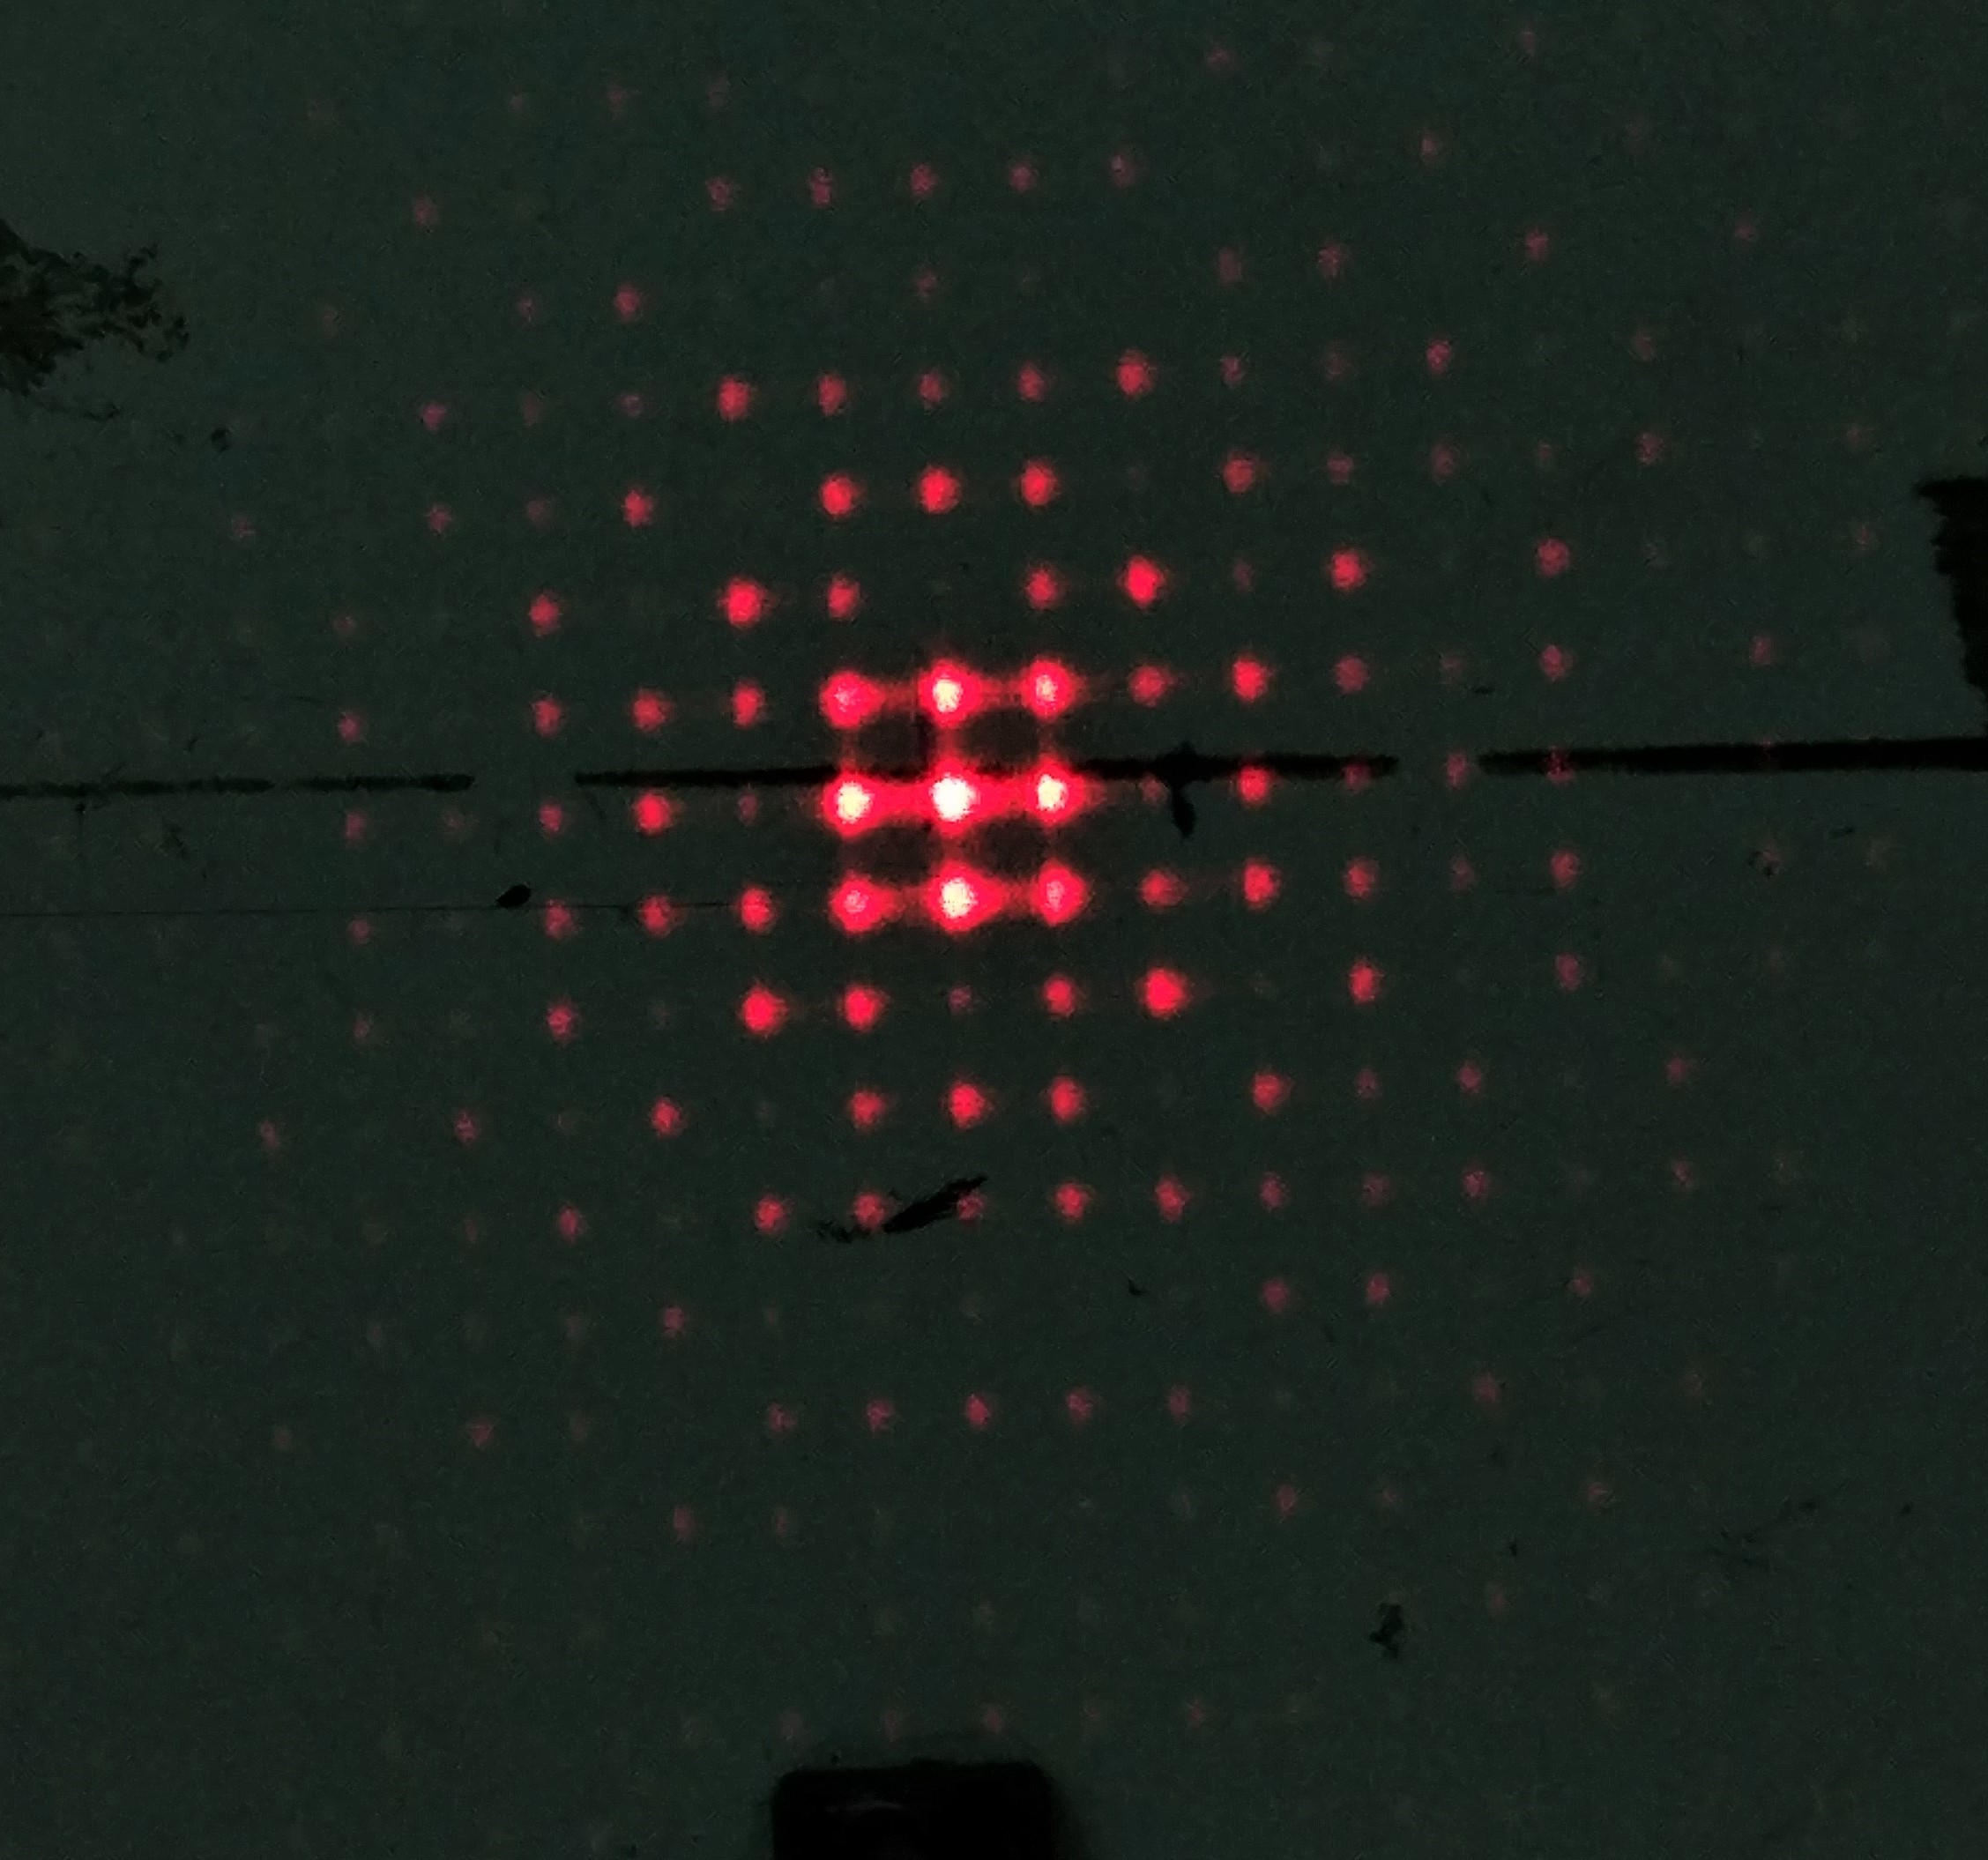
\includegraphics[width=0.27\linewidth]{ff.jpg}}\hfill
\subfigure[密堆方孔的衍射花样。]{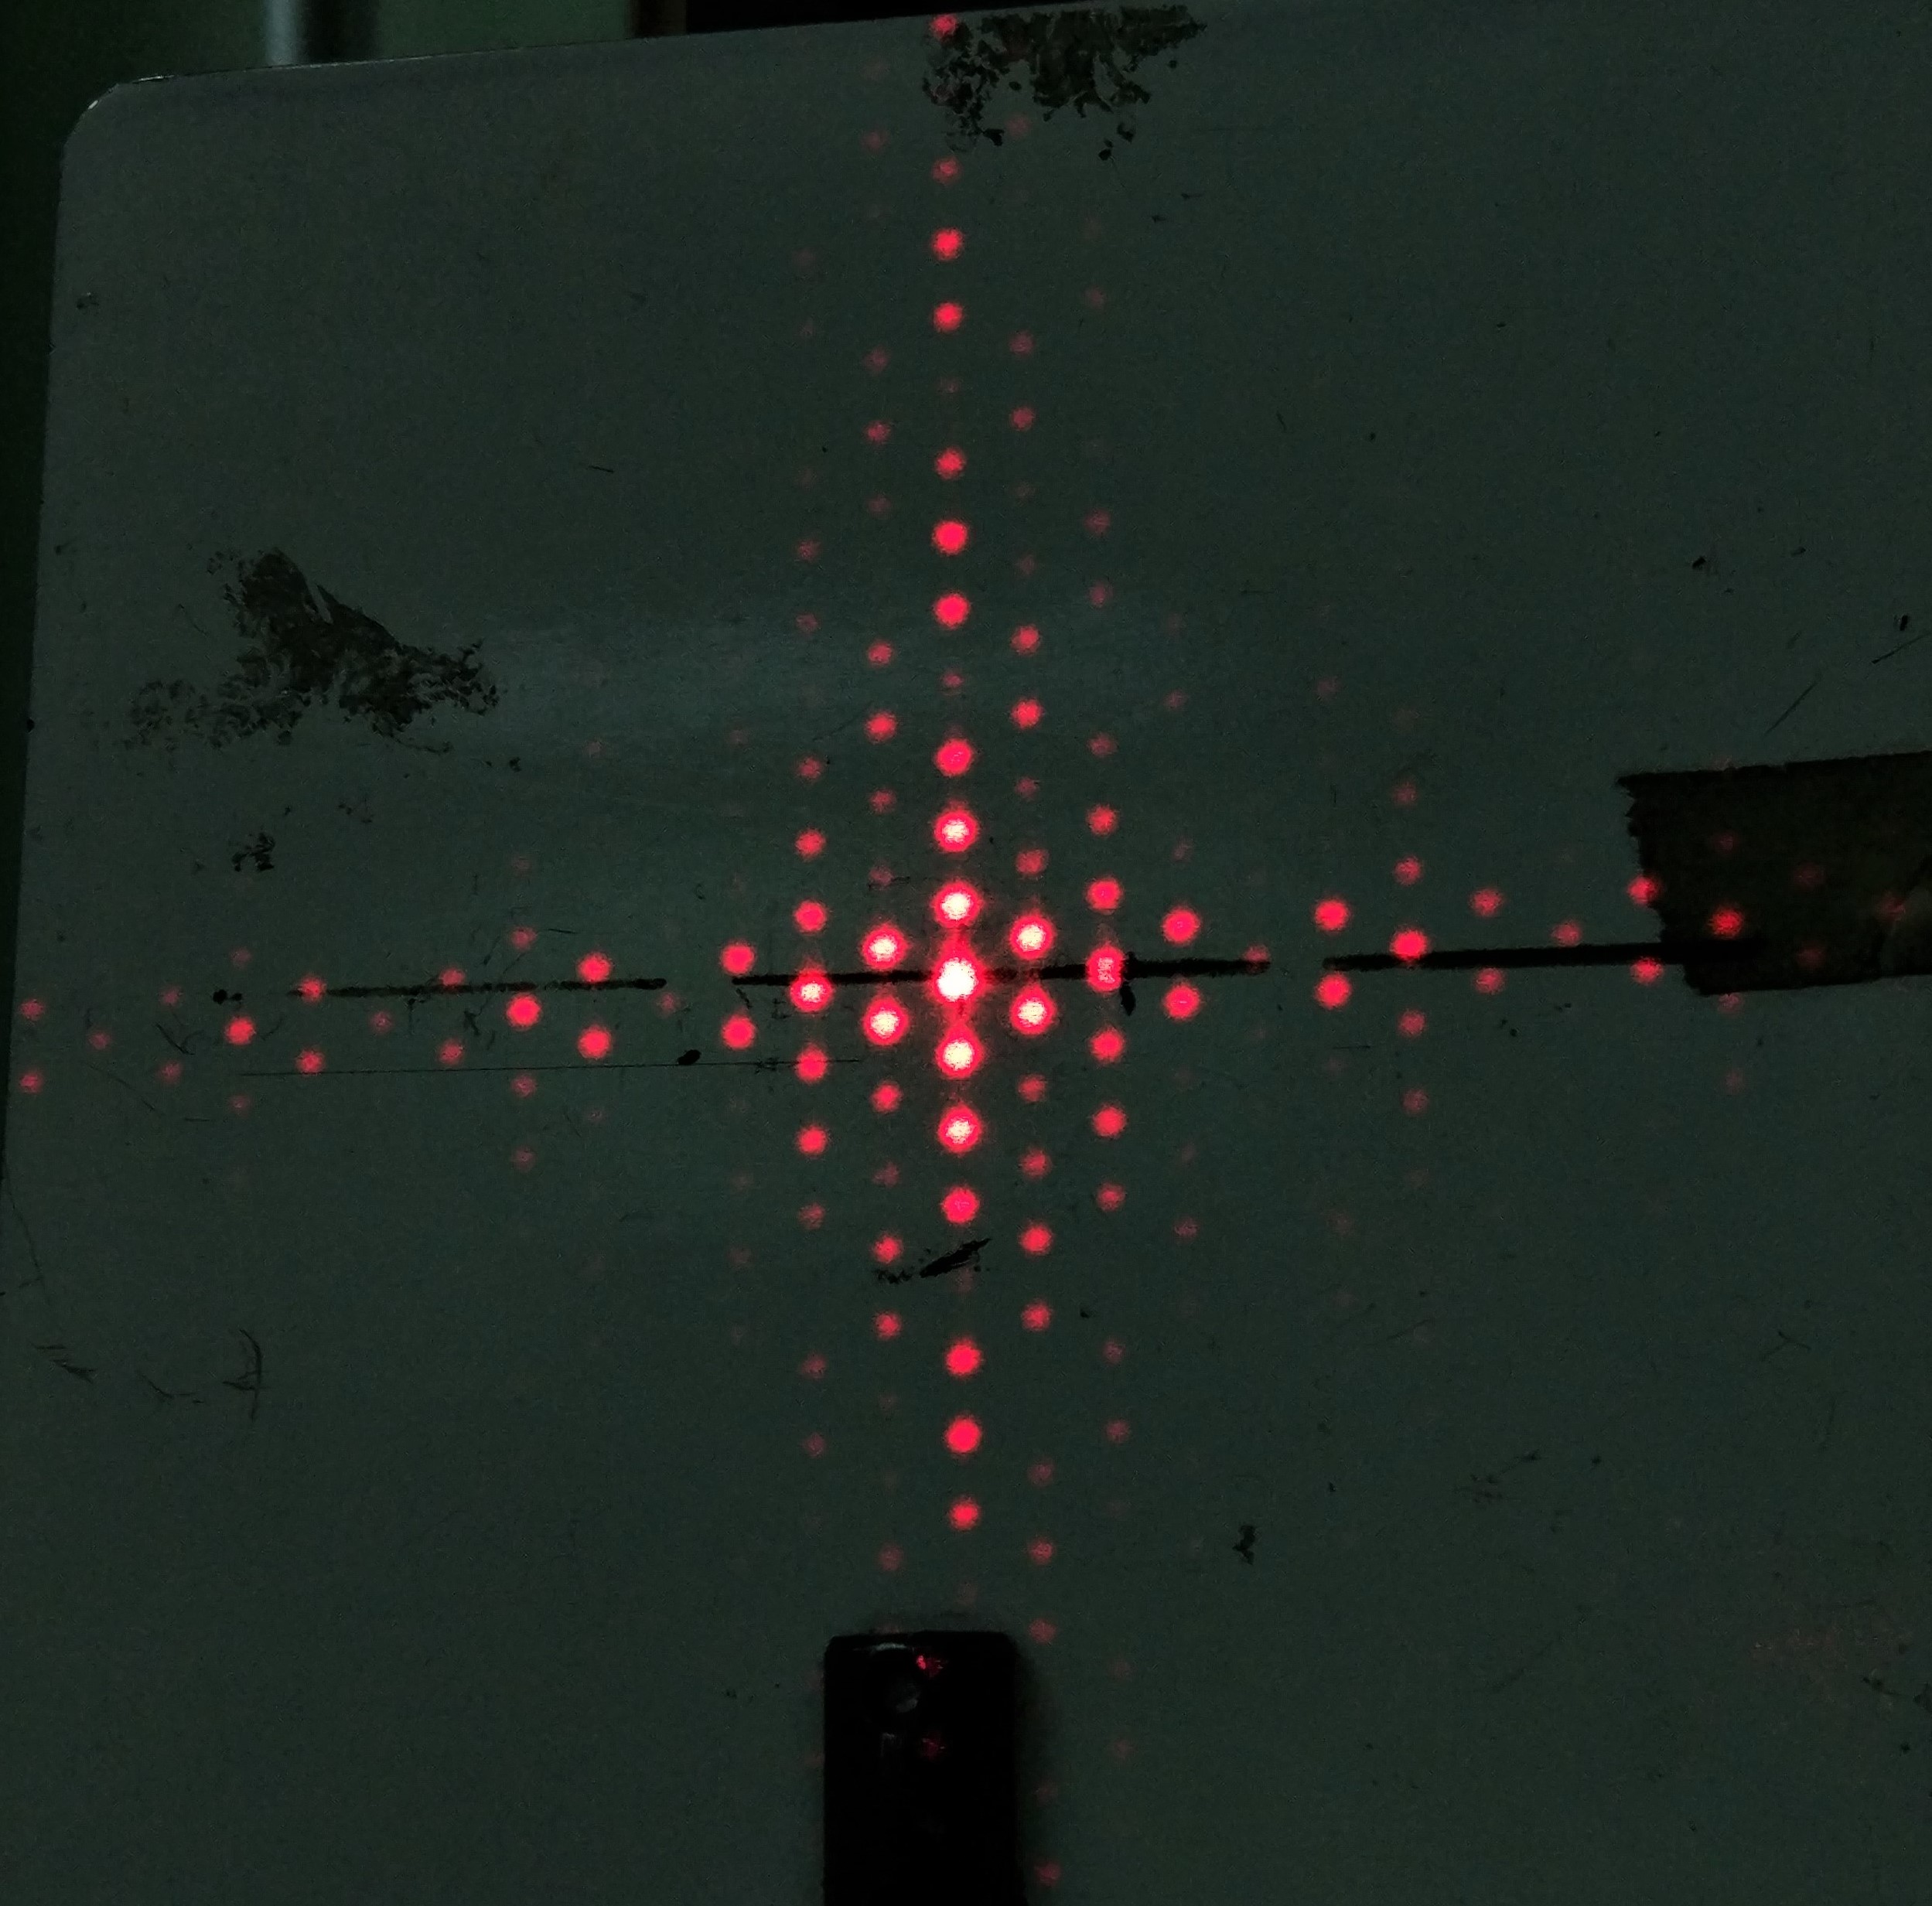
\includegraphics[width=0.25\linewidth]{yf.jpg}} \hfill
\subfigure[密堆圆孔的衍射花样。]{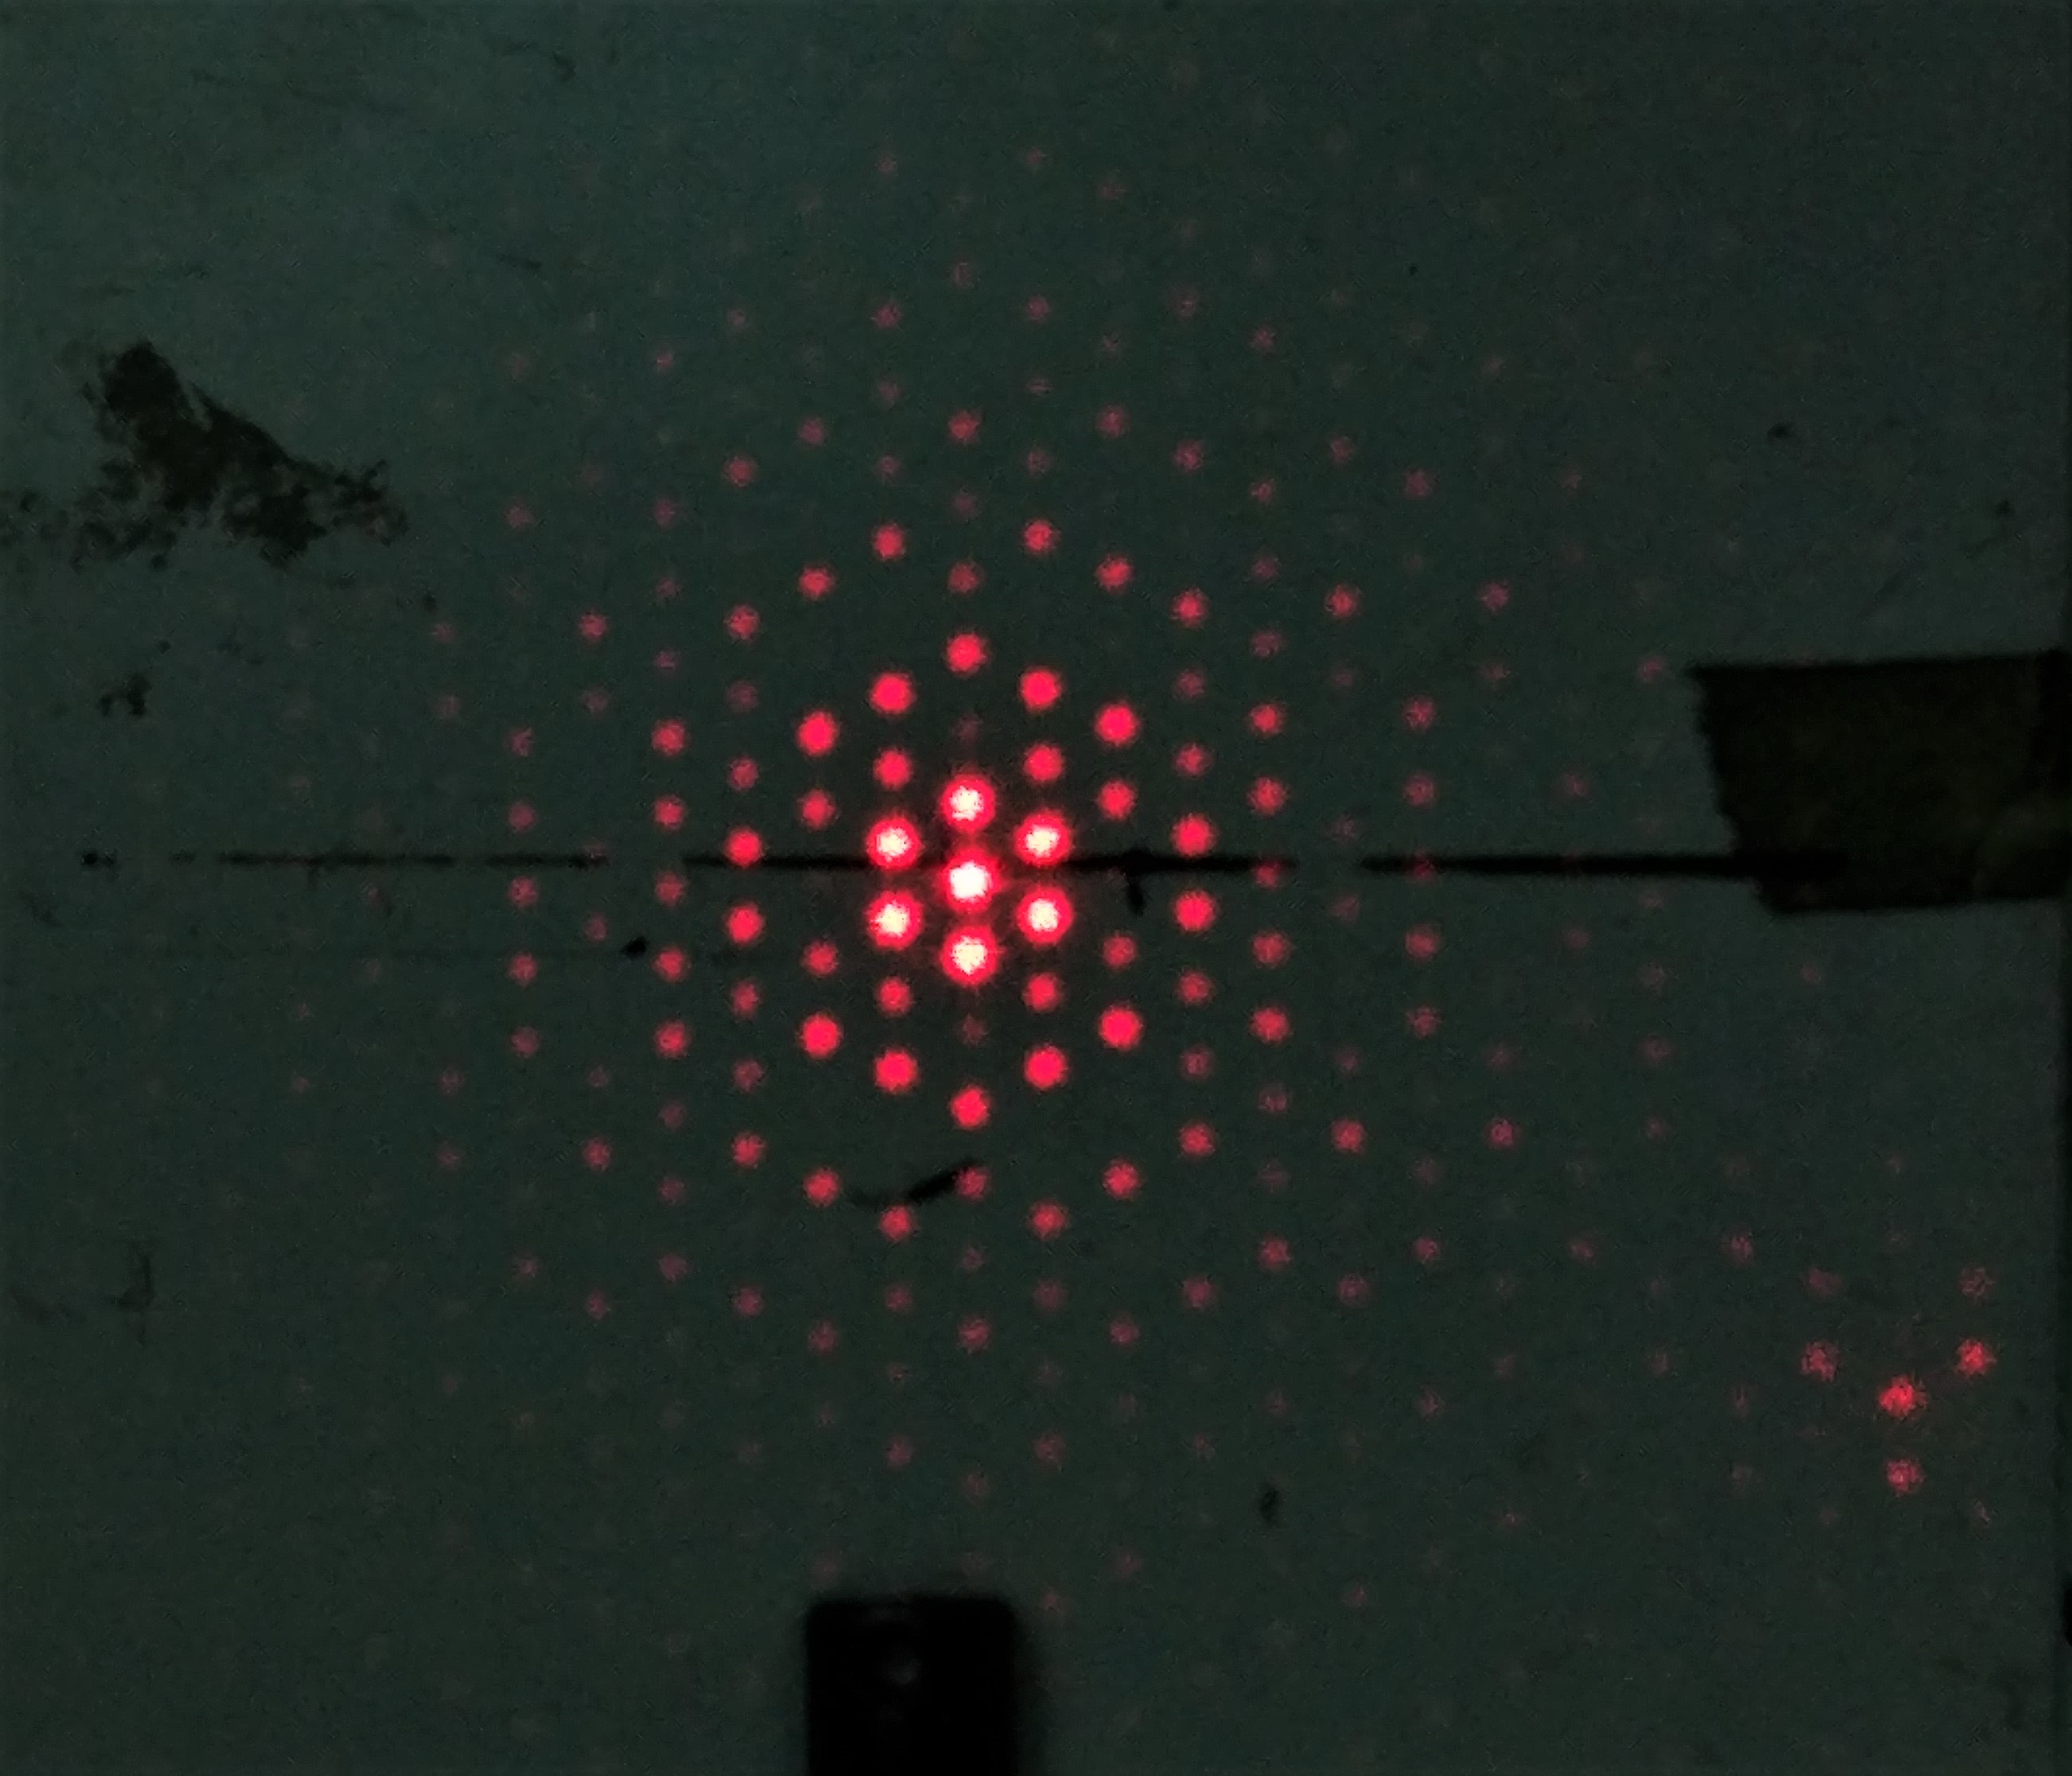
\includegraphics[width=0.3\linewidth]{ym.jpg}} \\
\subfigure[等边三角形孔的衍射花样。]{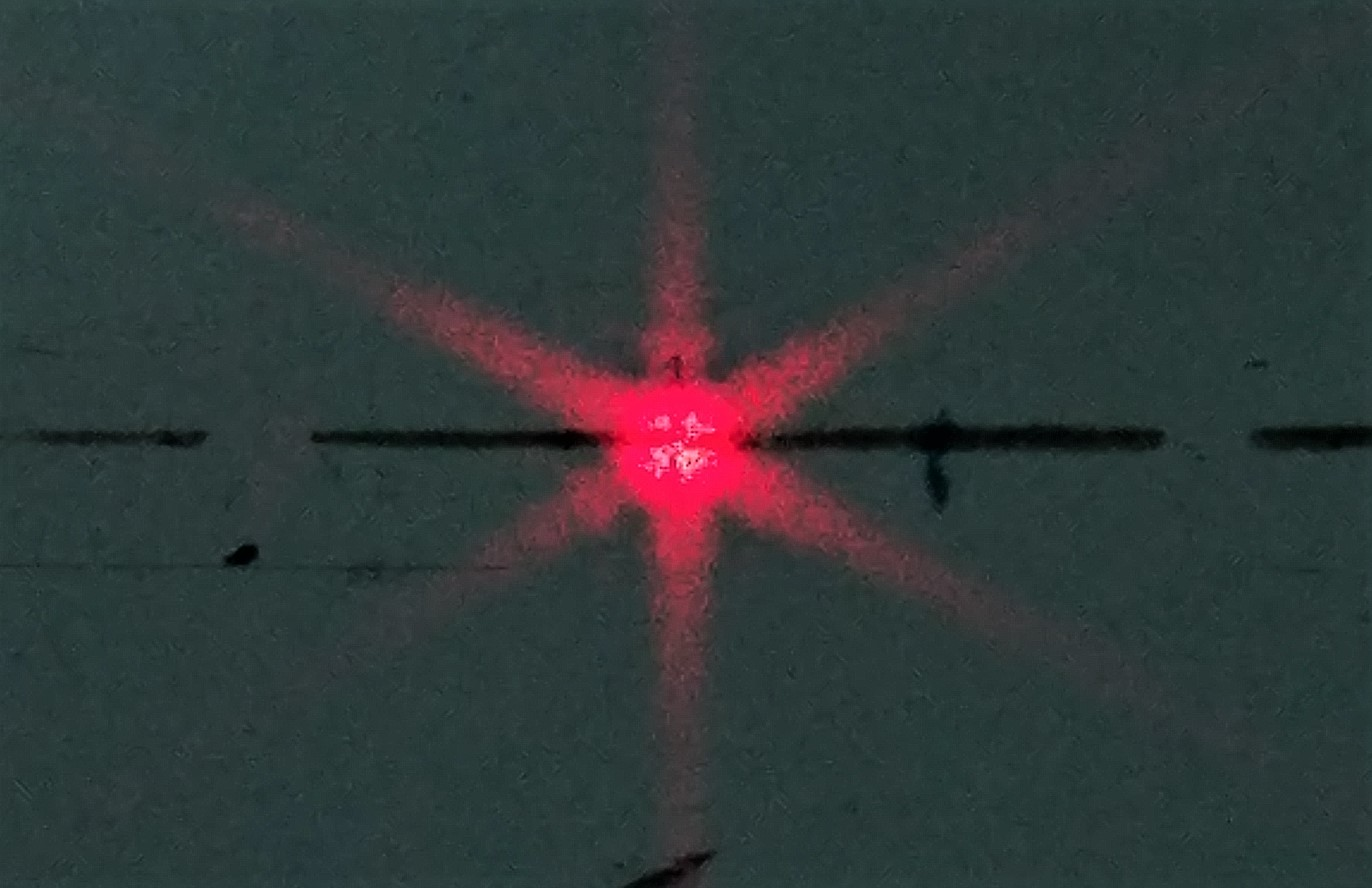
\includegraphics[width=0.4\linewidth]{db.jpg}}\hfill
\subfigure[等腰三角形孔的衍射花样。]{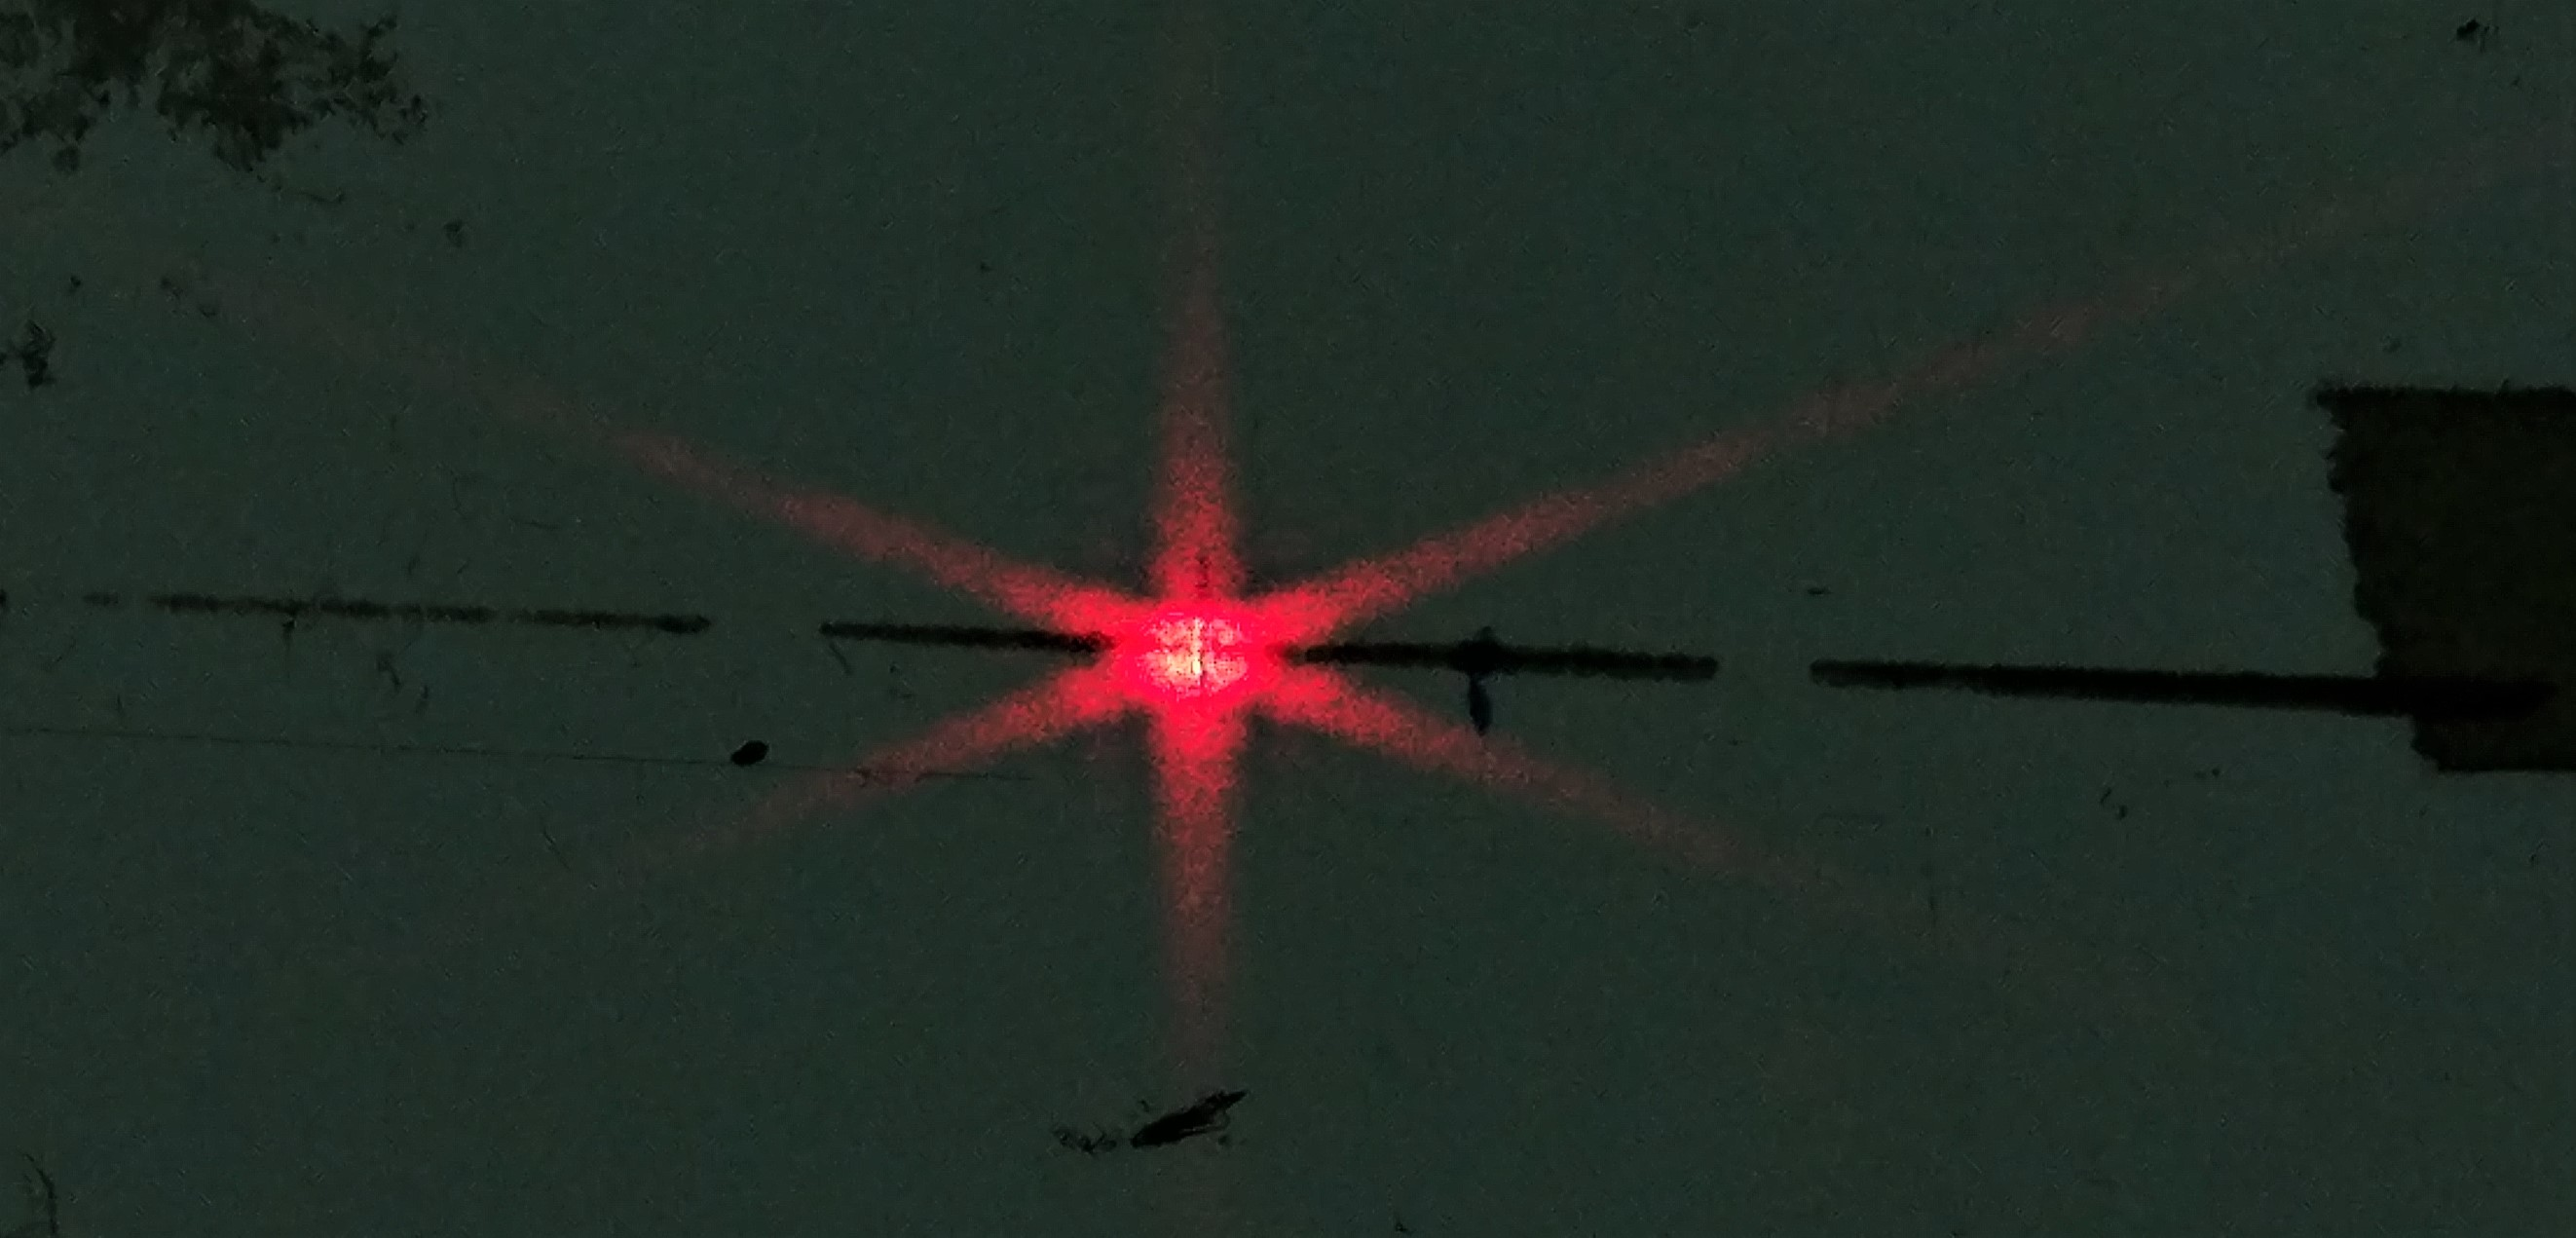
\includegraphics[width=0.54\linewidth]{dy.jpg}} \\
\end{figure}

\begin{figure}
\centering
\SetFigLayout{5}{1}
\subfigure[衍射物为单丝。]{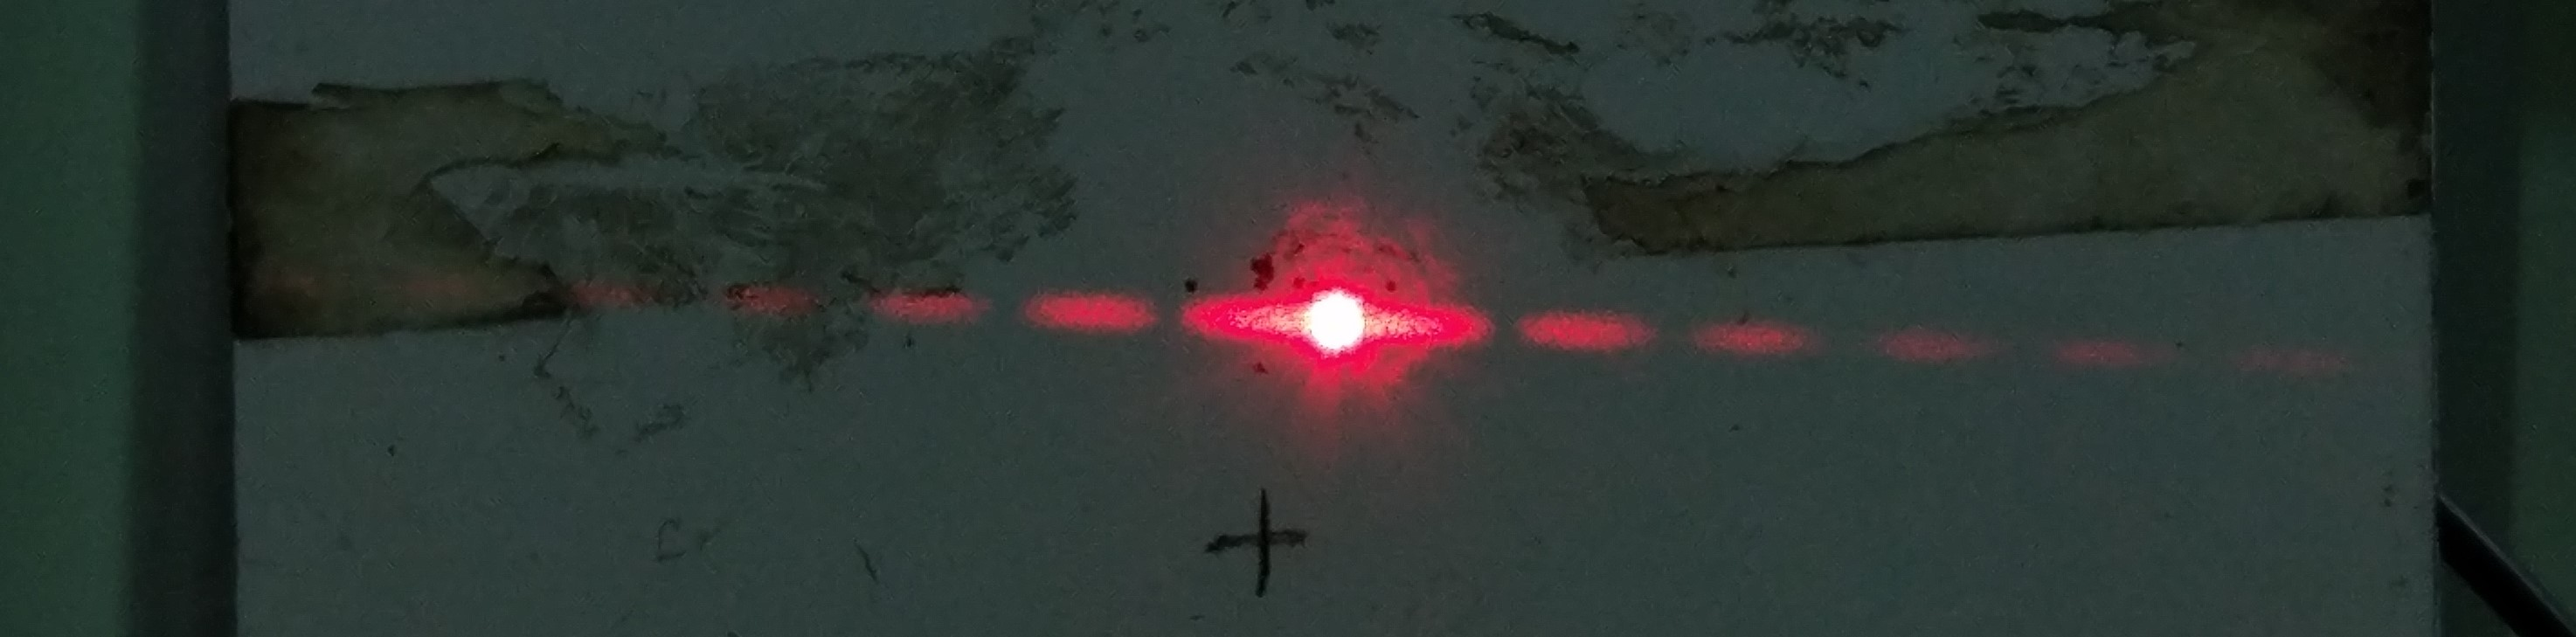
\includegraphics[width=\linewidth]{1.jpg}} \\
\subfigure[衍射物为双丝。]{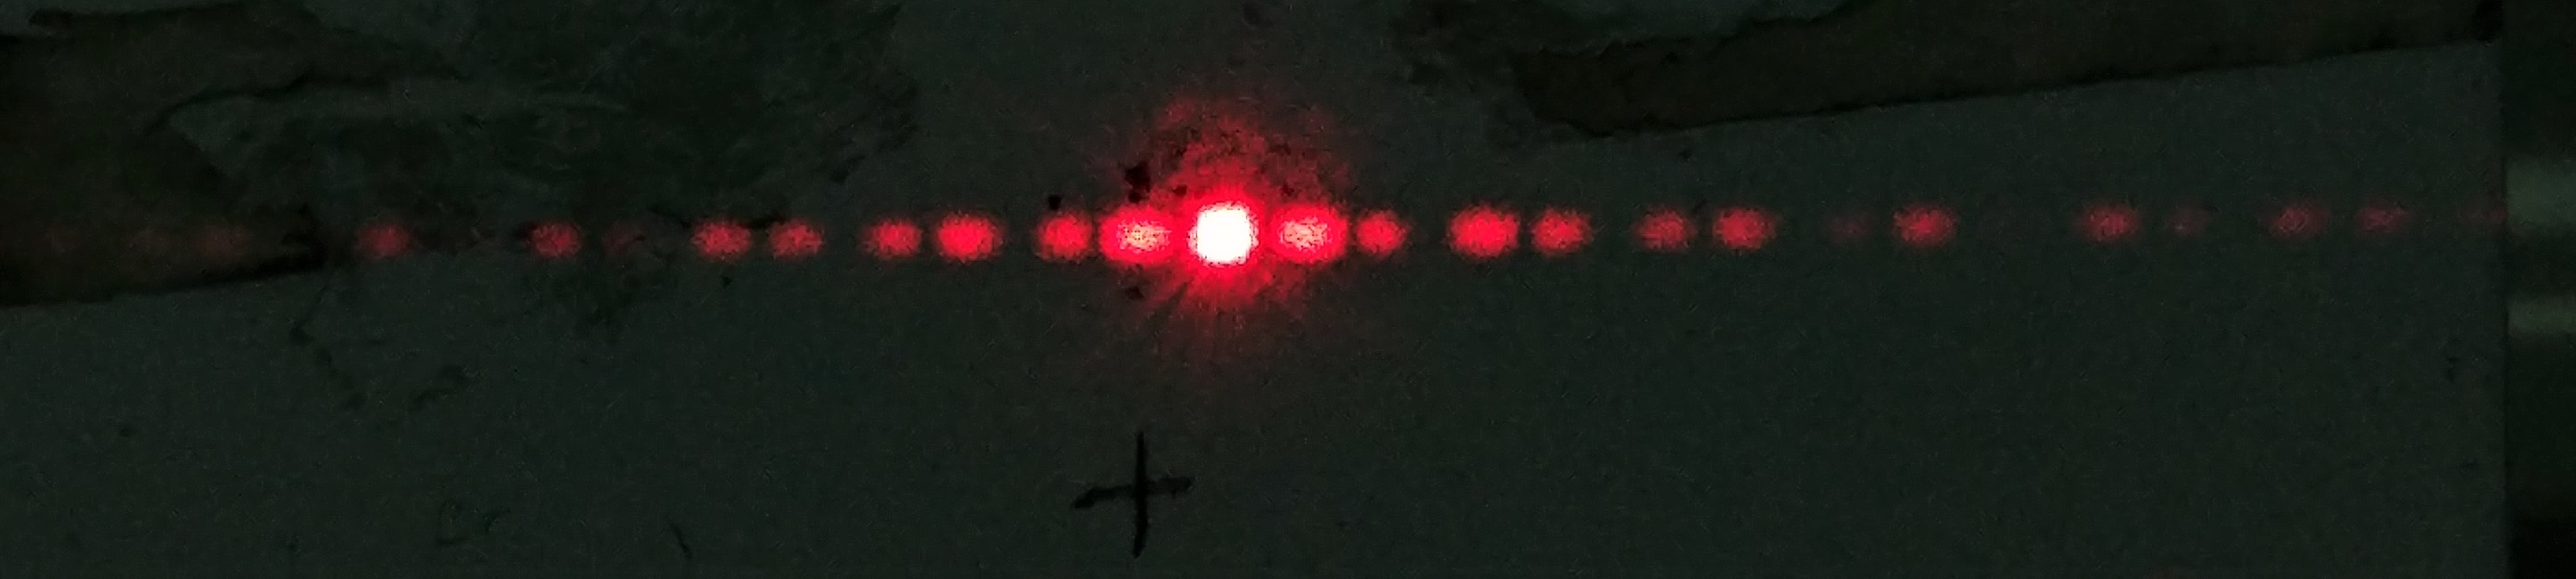
\includegraphics[width=\linewidth]{2.jpg}} \\
\subfigure[衍射物为三丝。]{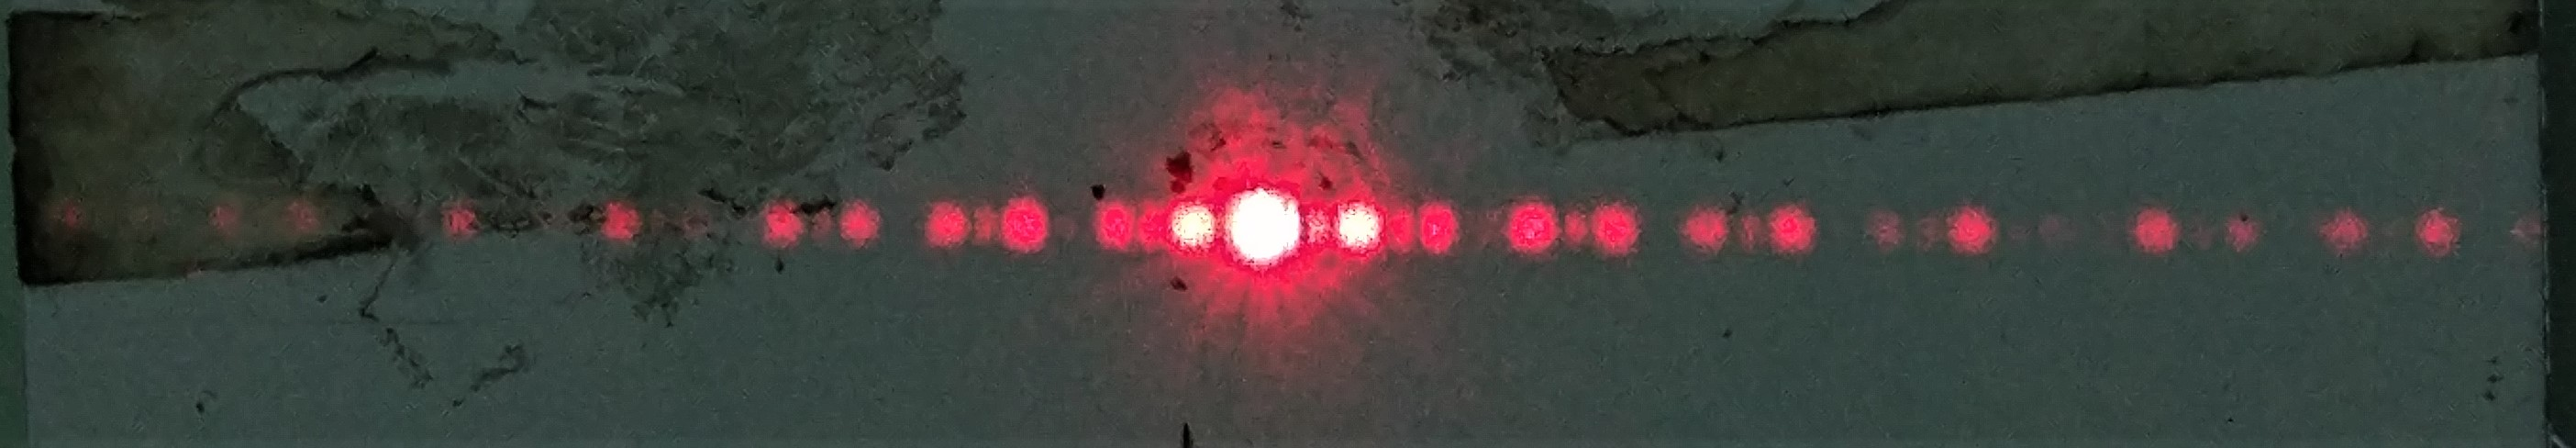
\includegraphics[width=\linewidth]{3.jpg}} \\
\subfigure[衍射物为四丝。]{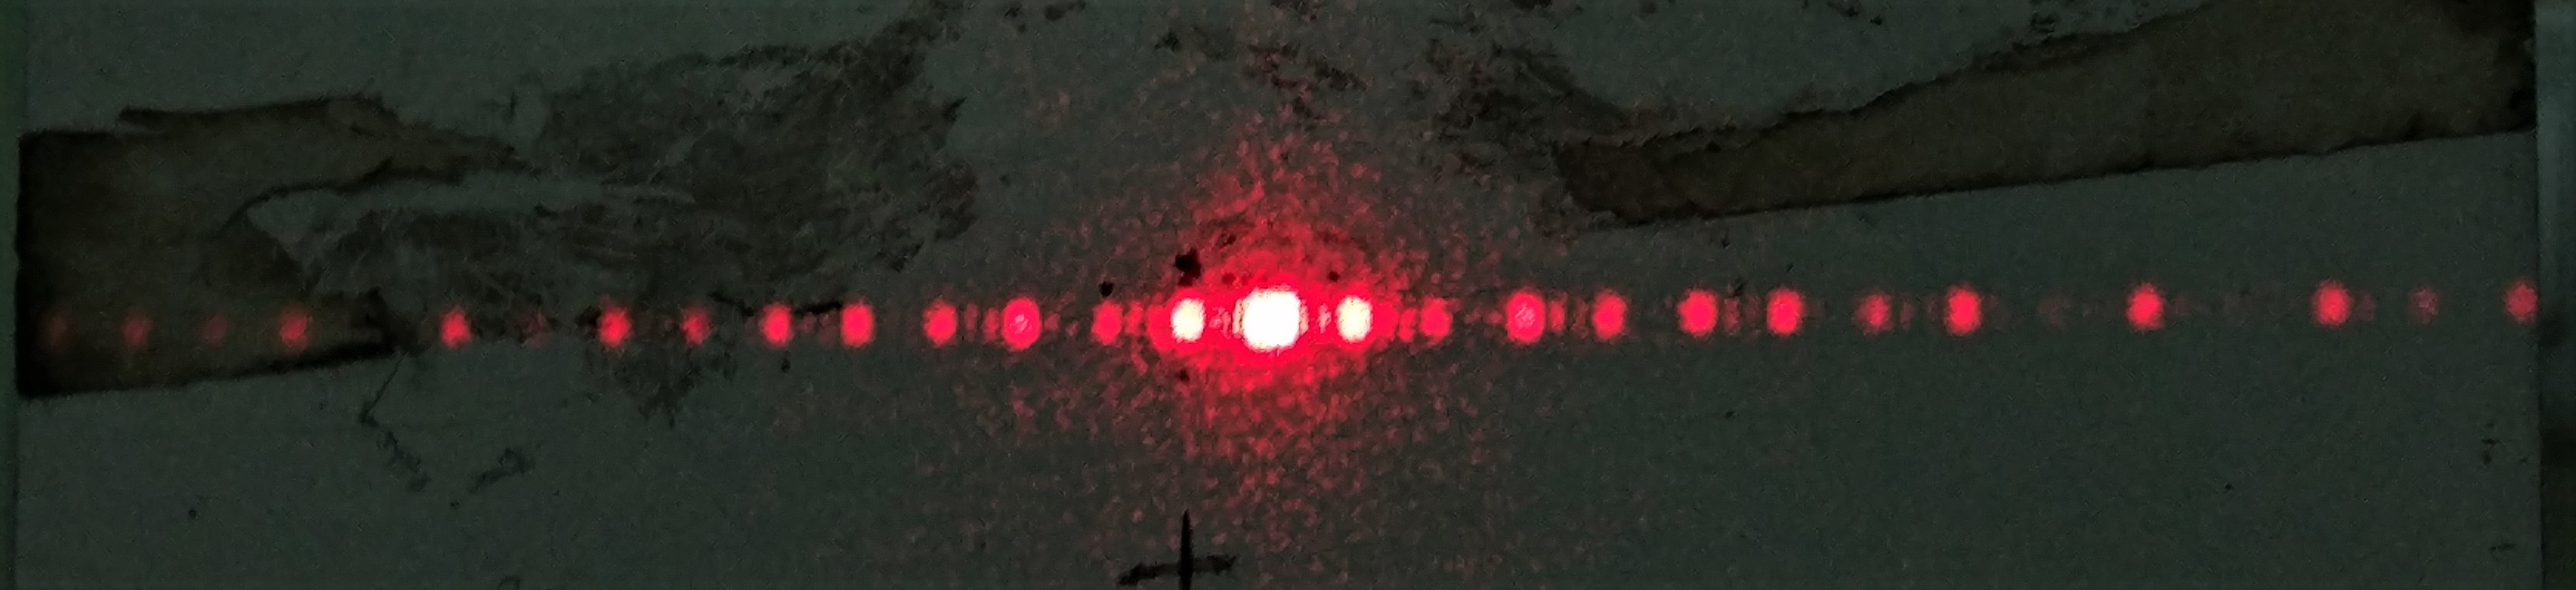
\includegraphics[width=\linewidth]{4.jpg}} \\
\subfigure[衍射物为五丝。]{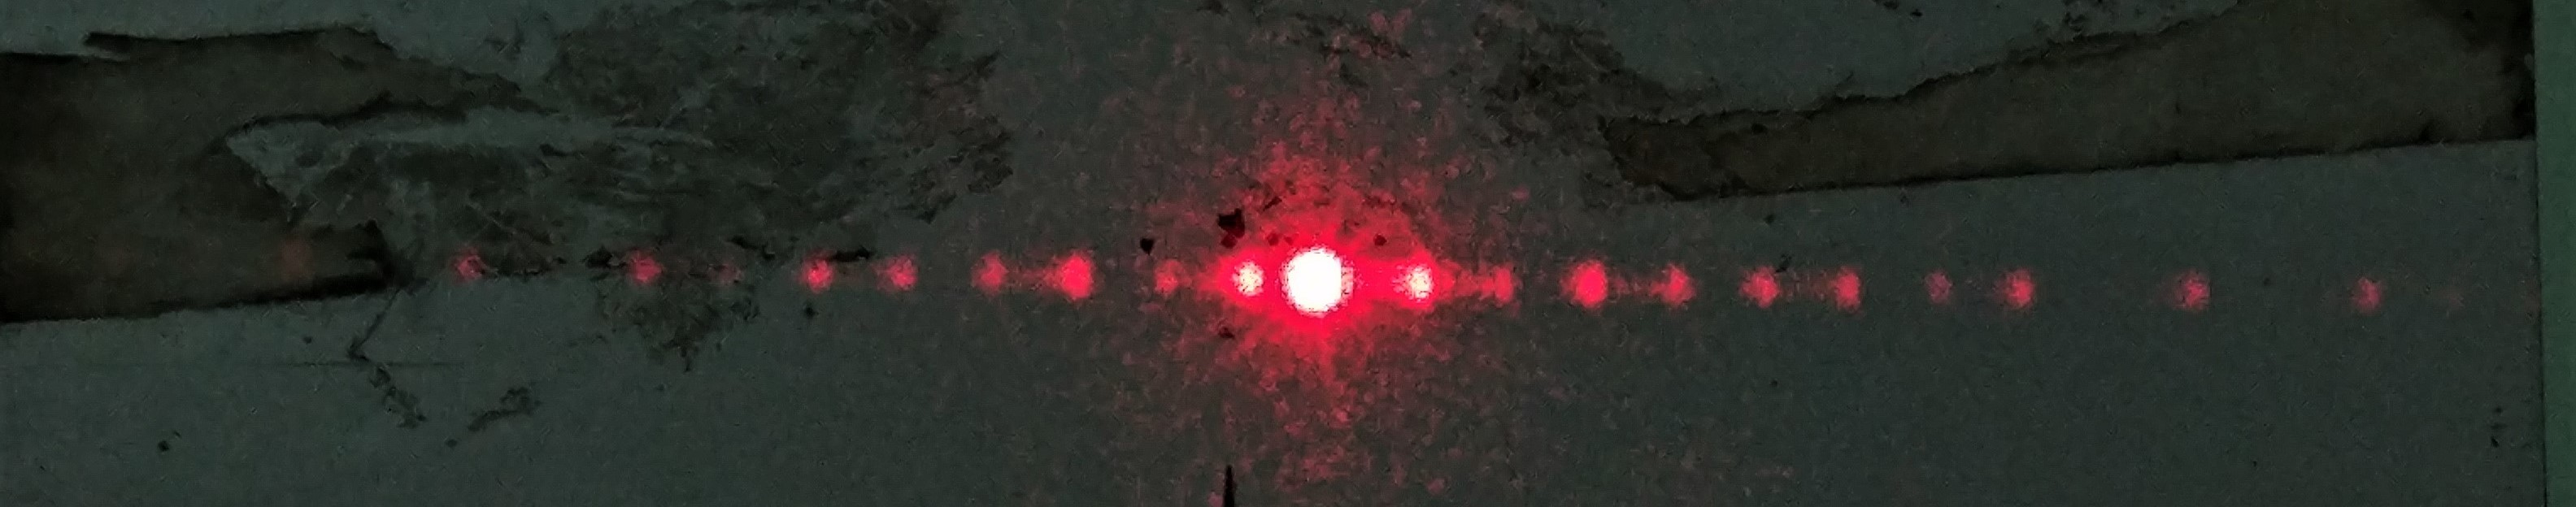
\includegraphics[width=\linewidth]{5.jpg}} \\
\caption{十个不同的衍射花样。}
\end{figure}

\begin{figure}
\centering
\SetFigLayout{3}{1}
\subfigure[单缝衍射的$I-x$图线(黑)与拟合曲线(红)。]{\includegraphics[width=\linewidth]{1slit.eps}} \\
\subfigure[双缝衍射的$I-x$图线(黑)与拟合曲线(红)。另绘制了一根按人工参数作出的拟合曲线(蓝色虚线),参见上文说明。]{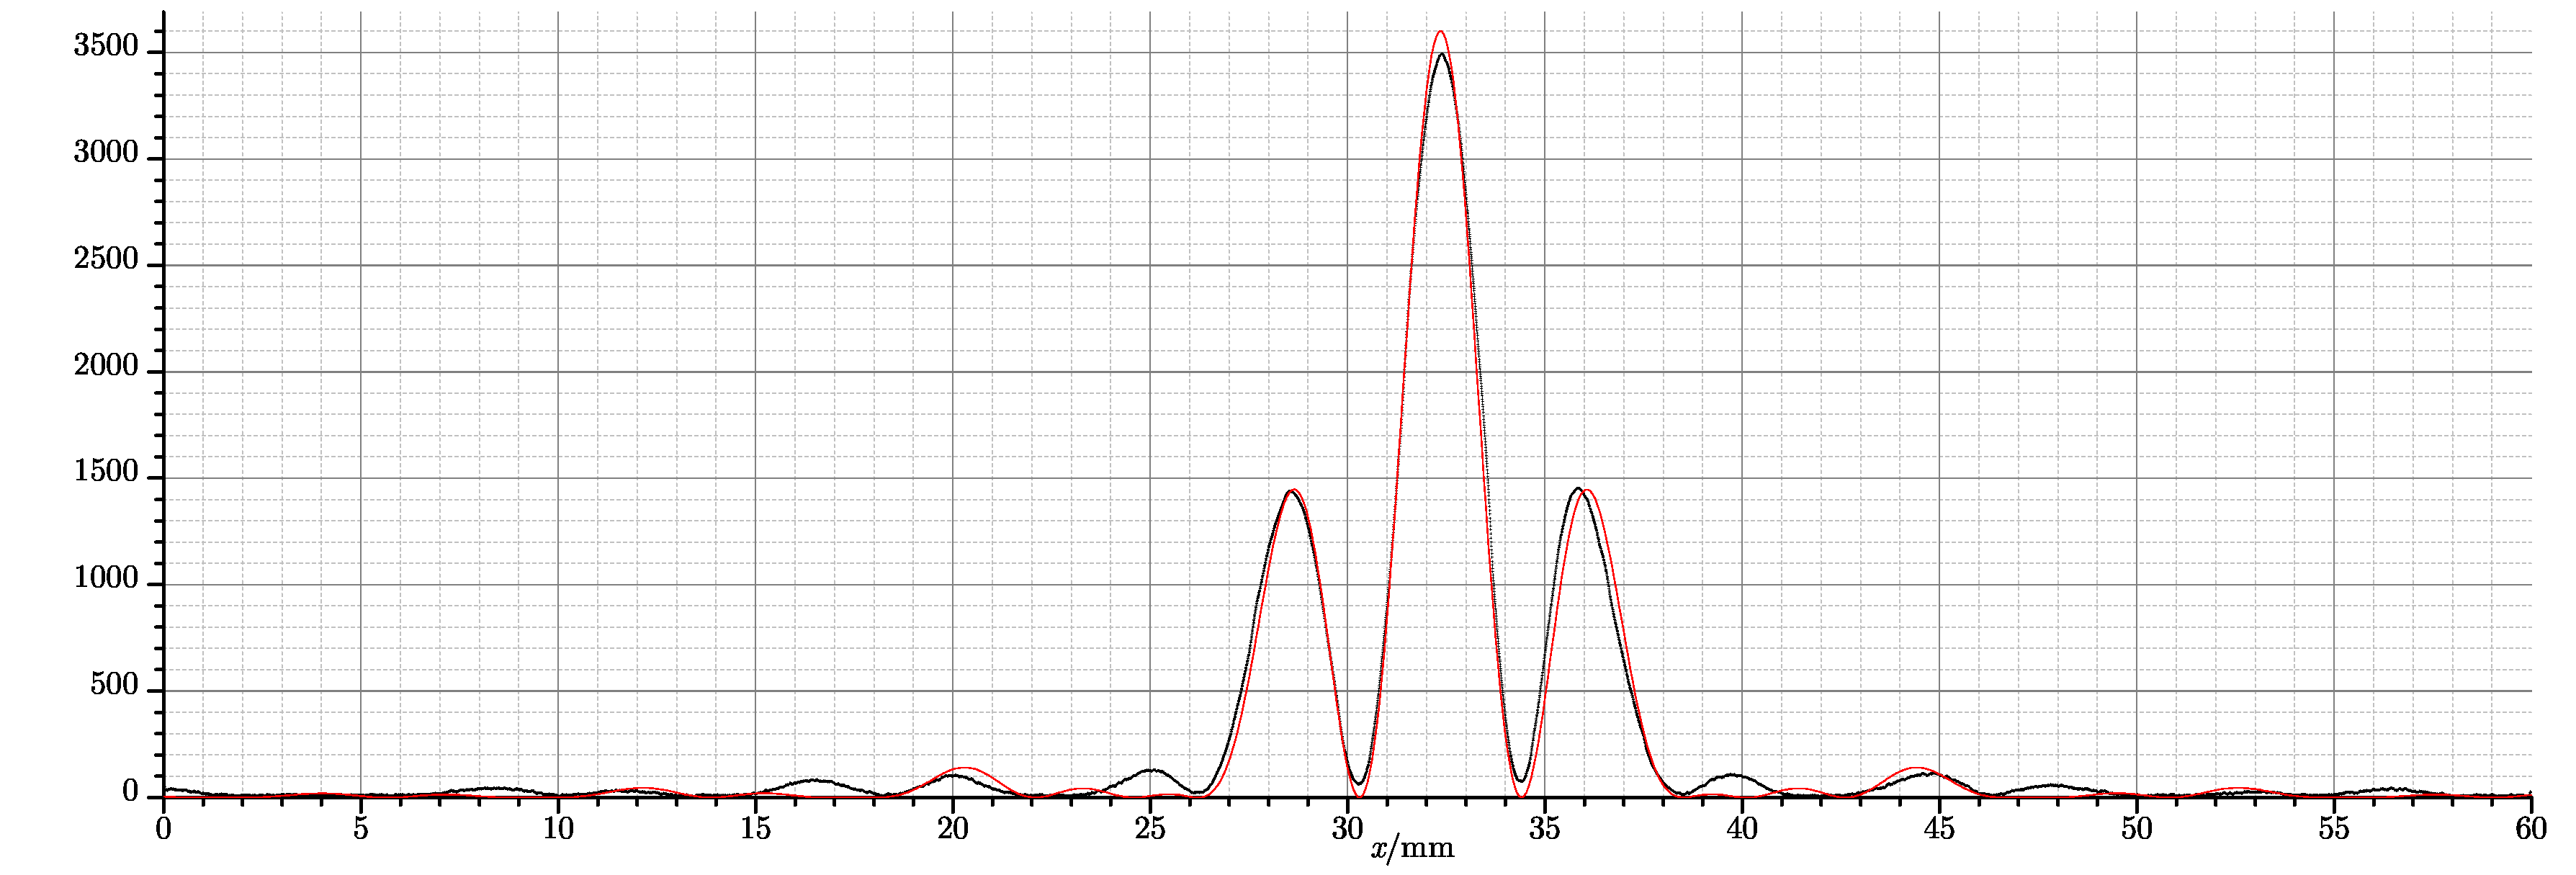
\includegraphics[width=\linewidth]{2slit.eps}} \\
\subfigure[四缝衍射的$I-x$图线(黑)与拟合曲线(红)。]{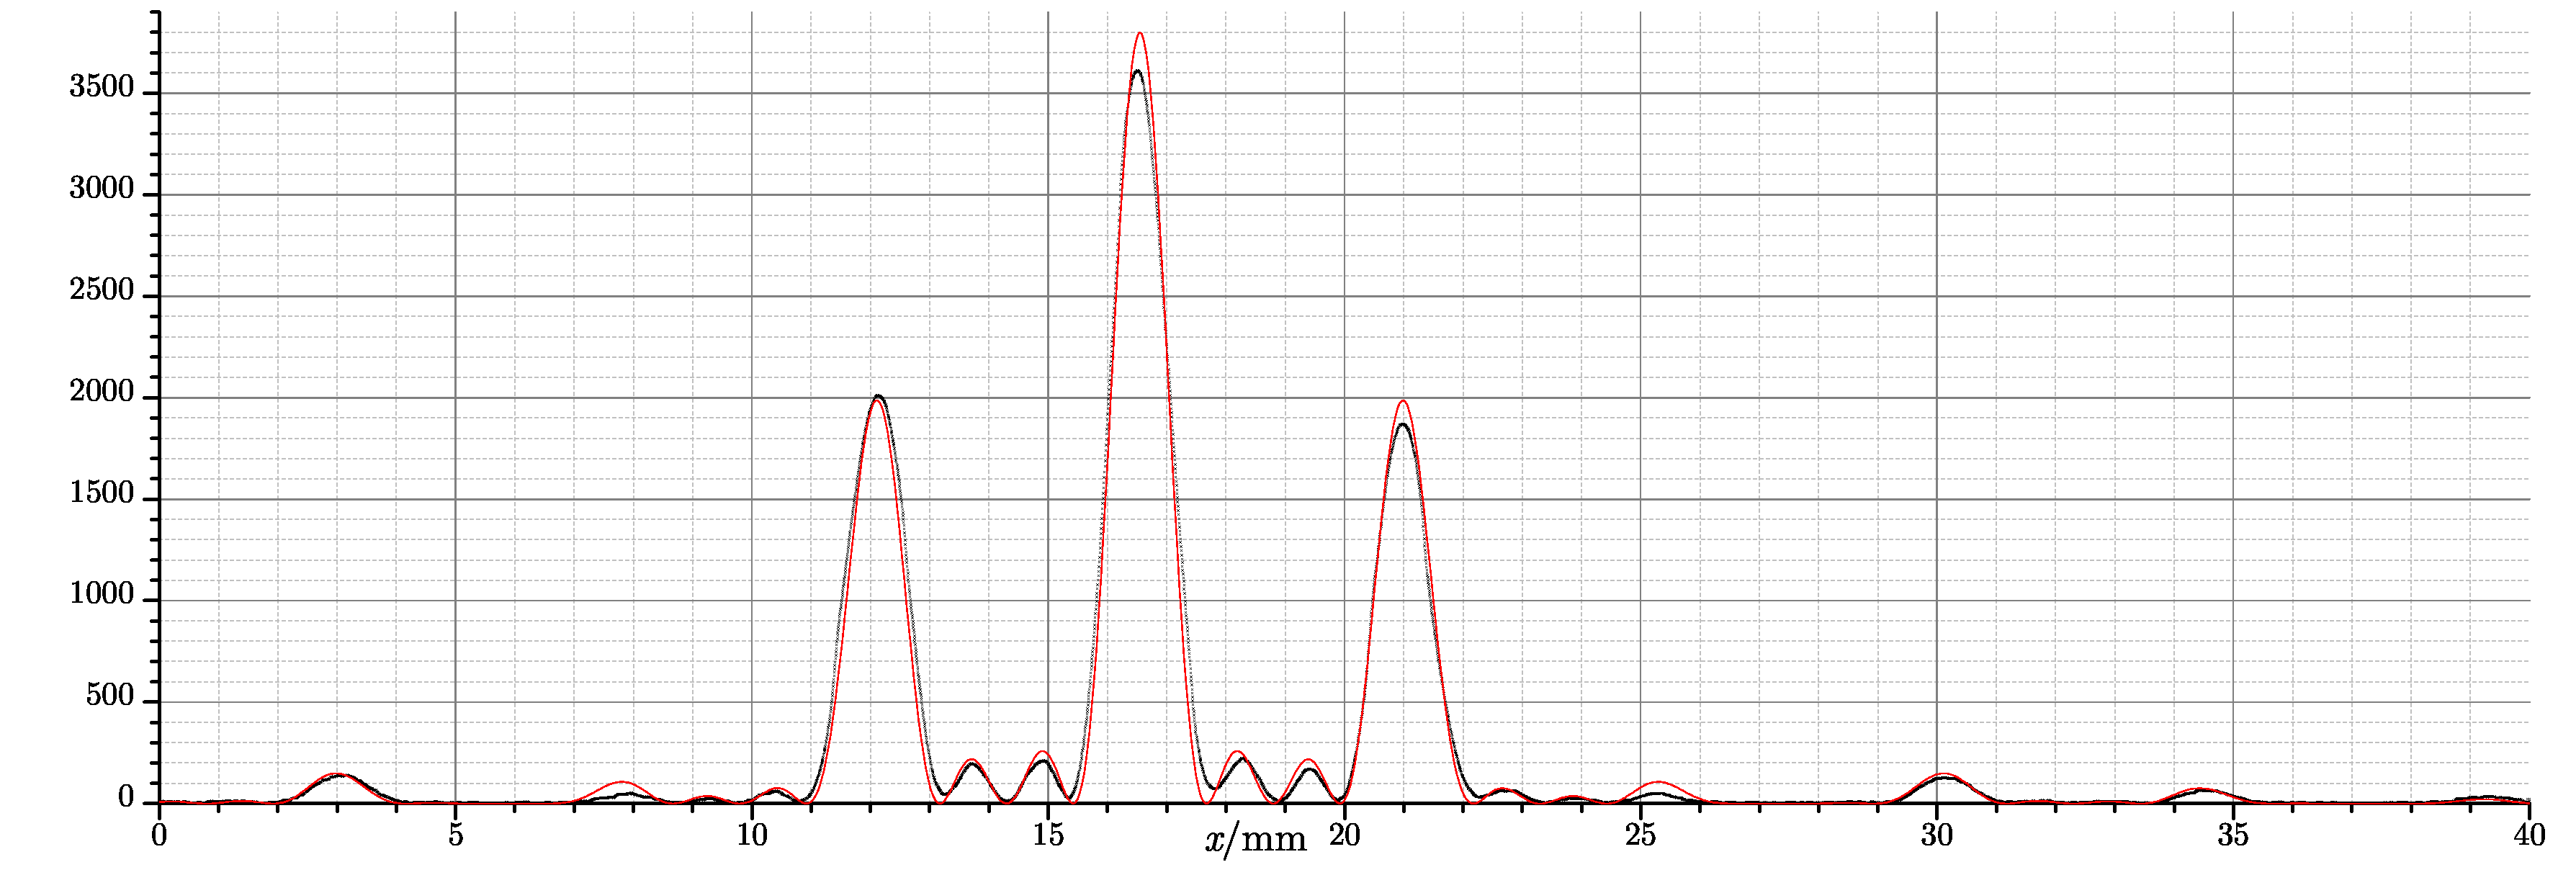
\includegraphics[width=\linewidth]{4slit.eps}} \\
\caption{传感器记录的光强数据。如果对原始数据感兴趣,或是觉得纸质黑白的图看不清的的话,可以访问\url{https://github.com/AgFlore/GeneralPhysicsLab/tree/master/Fraunhofer_diffraction}查看在线版。}
\end{figure}

\end{document}